\documentclass[border={1.5mm 0.6mm}]{standalone}
\usepackage[T1]{fontenc}
\usepackage{newtxtext,newtxmath}
\usepackage{xcolor}
\usepackage{tikz}
\usepackage{pgfplots}
\usepackage{amsmath}
\pgfplotsset{compat=1.18}
\usetikzlibrary{arrows.meta,calc,positioning,decorations.pathreplacing,fit,backgrounds,patterns,shapes.misc,shapes.geometric}
\usepgfplotslibrary{groupplots,fillbetween}
\definecolor{ink}{HTML}{111111}
\definecolor{accent}{HTML}{A8321F}
\definecolor{steel}{HTML}{1F4A7A}
\definecolor{midgray}{HTML}{6E6E6E}
\definecolor{lightgray}{HTML}{D9D9D9}
\newcommand{\figsize}{\fontsize{8}{9.6}\selectfont}
\newcommand{\smallsize}{\fontsize{7}{8.4}\selectfont}
\AtBeginDocument{\DeclareFontShape{OML}{ntxmi}{m}{it}{<-> ntxmi}{}\frenchspacing}
\pgfplotsset{
  every axis/.append style={
    axis line style={line width=0.45pt,ink},
    tick style={line width=0.4pt,ink},
    major tick length=3pt,
    minor tick length=1.6pt,
    tick align=inside,
    xtick pos=both,
    ytick pos=both,
    minor tick num=0,
    grid=none,
    label style={font=\figsize},
    tick label style={font=\figsize},
    legend style={font=\smallsize,draw=none,fill=none,inner sep=1pt,row sep=-0.5pt},
    legend cell align=left,
    xlabel near ticks,
    ylabel near ticks,
    /pgf/number format/1000 sep={\mbox{,}},
    scaled ticks=false,
    clip marker paths=true,
  },
  x25519/.style={ink,line width=0.5pt,solid,mark=*,mark size=1.0pt,mark options={solid,fill=ink,line width=0.2pt}},
  hybrid/.style={accent,line width=0.5pt,solid,mark=square*,mark size=0.95pt,mark options={solid,fill=accent,line width=0.2pt}},
  x25519open/.style={ink,only marks,mark=*,mark size=1.25pt,mark options={solid,fill=white,line width=0.45pt}},
  hybridopen/.style={accent,only marks,mark=square*,mark size=1.15pt,mark options={solid,fill=white,line width=0.45pt}},
}
\newcommand{\panel}[1]{{\figsize(#1)}}

\tikzset{
  blk/.style={draw=ink,line width=0.45pt,fill=white,minimum height=5mm,inner sep=0pt,align=center,font=\figsize},
  bl/.style={blk,minimum width=33mm},
  br/.style={blk,minimum width=35mm},
  arr/.style={-{Latex[length=3pt,width=2pt]},line width=0.45pt,ink},
  grp/.style={draw=midgray,line width=0.4pt,dash pattern=on 2.4pt off 1.8pt},
  org/.style={draw=ink,line width=0.45pt,fill=white},
  par/.style={draw=ink,line width=0.45pt,preaction={fill=white},pattern=north east lines,pattern color=midgray},
  brc/.style={decorate,decoration={brace,amplitude=1.3pt},line width=0.4pt,ink},
  sml/.style={font=\smallsize,inner sep=0pt,align=center},
  lab/.style={font=\figsize,inner sep=0pt,align=center},
}
\begin{document}
\figsize
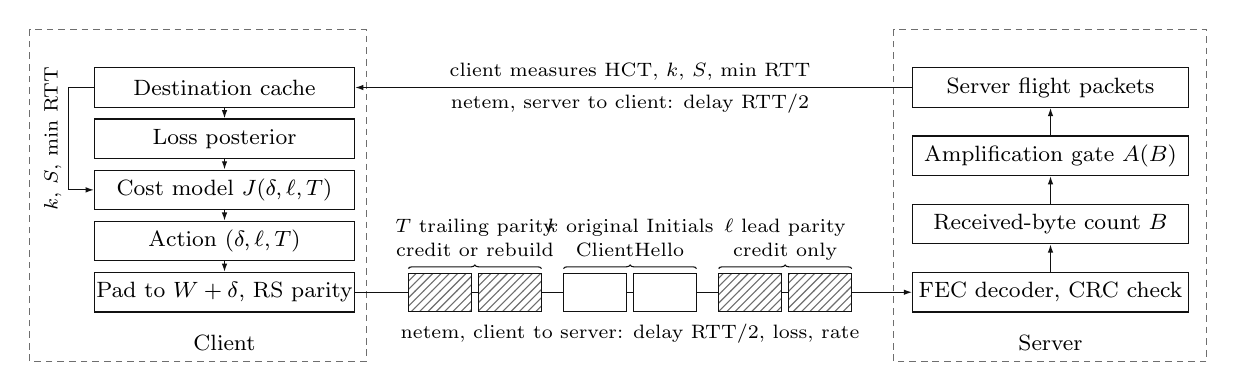
\begin{tikzpicture}[x=1mm,y=1mm]
\path (0,0) rectangle (150,42.60);
\draw[grp] (0.25,0.25) rectangle (43.00,42.35);
\draw[grp] (110.00,0.25) rectangle (149.75,42.35);
\node[lab] at (25.00,2.6) {Client};
\node[lab] at (129.90,2.6) {Server};
\node[bl] (dc) at (25.00,35.000) {Destination cache};
\node[bl] (lp) at (25.00,28.500) {Loss posterior};
\node[bl] (cm) at (25.00,22.000) {Cost model $J(\delta,\ell,T)$};
\node[bl] (ac) at (25.00,15.500) {Action $(\delta,\ell,T)$};
\node[bl] (pe) at (25.00,9.000) {Pad to $W+\delta$, RS parity};
\draw[arr] (dc.south) -- (lp.north);
\draw[arr] (lp.south) -- (cm.north);
\draw[arr] (cm.south) -- (ac.north);
\draw[arr] (ac.south) -- (pe.north);
\draw[arr] (dc.west) -- (5.2,35.000) -- (5.2,22.000) -- (cm.west);
\node[sml,rotate=90] at (3.2,28.500) {$k$, $S$, min RTT};
\node[br] (dec) at (129.90,9.000) {FEC decoder, CRC check};
\node[br] (rb) at (129.90,17.667) {Received-byte count $B$};
\node[br] (gt) at (129.90,26.333) {Amplification gate $A(B)$};
\node[br] (tf) at (129.90,35.000) {Server flight packets};
\draw[arr] (dec.north) -- (rb.south);
\draw[arr] (rb.north) -- (gt.south);
\draw[arr] (gt.north) -- (tf.south);
\draw[arr] (pe.east) -- (dec.west);
\draw[arr] (tf.west) -- (dc.east);
\draw[par] (48.350,6.600) rectangle (56.350,11.400);
\draw[par] (57.250,6.600) rectangle (65.250,11.400);
\draw[org] (68.050,6.600) rectangle (76.050,11.400);
\draw[org] (76.950,6.600) rectangle (84.950,11.400);
\draw[par] (87.750,6.600) rectangle (95.750,11.400);
\draw[par] (96.650,6.600) rectangle (104.650,11.400);
\draw[brc] (48.350,12.000) -- (65.250,12.000);
\draw[brc] (68.050,12.000) -- (84.950,12.000);
\draw[brc] (87.750,12.000) -- (104.650,12.000);
\node[sml,anchor=base] at (56.800,16.600) {$T$ trailing parity};
\node[sml,anchor=base] at (56.800,13.500) {credit or rebuild};
\node[sml,anchor=base] at (76.500,16.600) {$k$ original Initials};
\node[sml,anchor=base] at (76.500,13.500) {ClientHello};
\node[sml,anchor=base] at (96.200,16.600) {$\ell$ lead parity};
\node[sml,anchor=base] at (96.200,13.500) {credit only};
\node[sml,anchor=north] at (76.500,5.000) {netem, client to server: delay RTT/2, loss, rate};
\node[sml,anchor=north] at (76.500,34.200) {netem, server to client: delay RTT/2};
\node[sml,anchor=south] at (76.500,35.800) {client measures HCT, $k$, $S$, min RTT};
\pgfresetboundingbox
\path (0,0) rectangle (150,42.60);
\end{tikzpicture}
\end{document}
